\documentclass{article}
\usepackage{hyperref}
\usepackage{graphicx}
\begin{document}
	\section*{Lsg Vorschlag ADS Ü01 A2 Maximilian Maag}
	\subsection*{Aufgabe 1}
	Die folgende Darstellung skizziert die Situation im Speicher nach den ersten 5 Zeilen. Die jeweilige Nummer Zeile ist als Zahl neben dem Objekt aufgetragen. \\ \\
	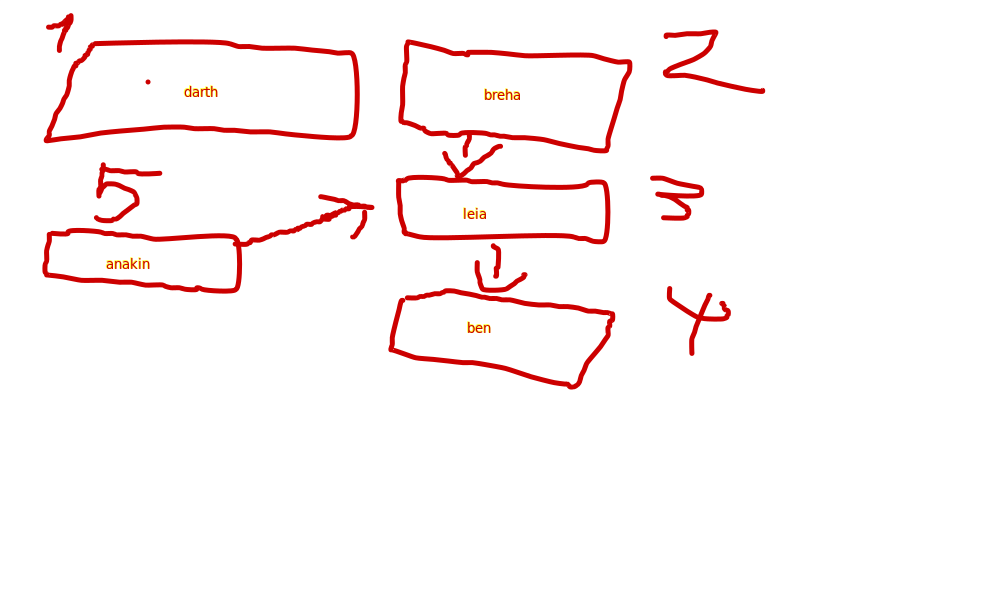
\includegraphics[width=\linewidth]{A2B01.png}
	\subsection*{Aufgabe 2}
	\begin{itemize}
		\item Für das Objekt leia wird das Feld parent auf den neuen Wert "darth" gesetzt.
		\item Für das Objekt leia wird das Feld name auf den Wert "Vader" gesetzt.
	\end{itemize}
	\subsection*{Aufgabe 3}
	\begin{itemize}
		\item true
		\item organa
		\item organa
		\item null
		\item wift eine Exception.
	\end{itemize}
\end{document}